Before extending gMark, we examine the state-of-the-art in synthetic graph generation to see what other techniques exist and what the strengths and weaknesses of the various methods are.

\section{LDBC}
The LDBC (Linked Data Benchmark Council) uses a benchmark called the Social Network Benchmark \cite{Erling2015TheBenchmark, LDBCBenchmark}. To generate the scaleable synthetic data sets necessary for this benchmark, the LDBC uses a tool called datagen. The LDBC wants to use datasets with sensible PageRank outcomes and graph clustering structure, so their approach is to design a data model and generate data sets within this fixed model. Their data model has fixed node types such as "Person", "University", "Country" and the attributes of nodes of these types are generated using pre-defined functions (age) and dictionaries (name).
The advantage of using a fixed data model is that advanced correlations can be generated that would be difficult to generate in the generic case where nothing about the model is assumed. For example, datagen ensures that persons are more likely to be connected in the social network when they are similar. They accomplish this by pre-defining a similarity metric between nodes of type Person and by then grouping persons having similar scores together when generating edges. This ensures that persons living in the same location, studying at the same university or having similar interests are more likely to be connected in the network.
A few other correlations that datagen ensures are sensible are person name with respect to location and gender, person email address with respect to the popularity of the email's domain name, IP address with respect to location and duration of employment with respect to age.
The result is that datagen can generate graphs containing realistic data up to correlations between attribute values, but the clear downside is that it can only generate graphs with one specific fixed schema. Graphgen cannot generate graphs based on an arbitrary schema.

\section{Kronecker graphs}
Kronecker graphs are based around the Kronecker product. The Kronecker product is an operation on two matrices as shown in definition \ref{def:kronecker_product}.

\begin{defn}
    $A \otimes B =$
    \begin{bmatrix}
        a_{11}\textbf{B} \dots a_{1n}\textbf{B} \\
        \vdots \ddots \vdots \\
        a_{m1}\textbf{B} \dots a_{mn}\textbf{B}
    \end{bmatrix}
    for matrices A, B. \cite{Edu2010KroneckerLeskovec}
    \label{def:kronecker_product}
\end{defn}

The Kronecker product of two graphs is then the Kronecker product of their corresponding adjacency matrices \cite{Edu2010KroneckerLeskovec}. This can be used to generate synthetic graphs as follows. Firstly, take or randomly generate an initiator graph. Take the Kronecker product of this graph with itself to produce a new graph. One can then keep iteratively taking the Kronecker product of the resulting graph with itself in order to produce new bigger graphs.
The reasoning behind this process is to recursively create self-similar graphs that exhibit the densification power law, for which the Kronecker product is suitable. The recursive self-similar structure can be observed in figure \ref{fig:kronecker_matrix}. Intuitively, real-world communities also recursively create new communities, which is how Kronecker graphs mimic real-world social networks.

\begin{figure}[!ht]
    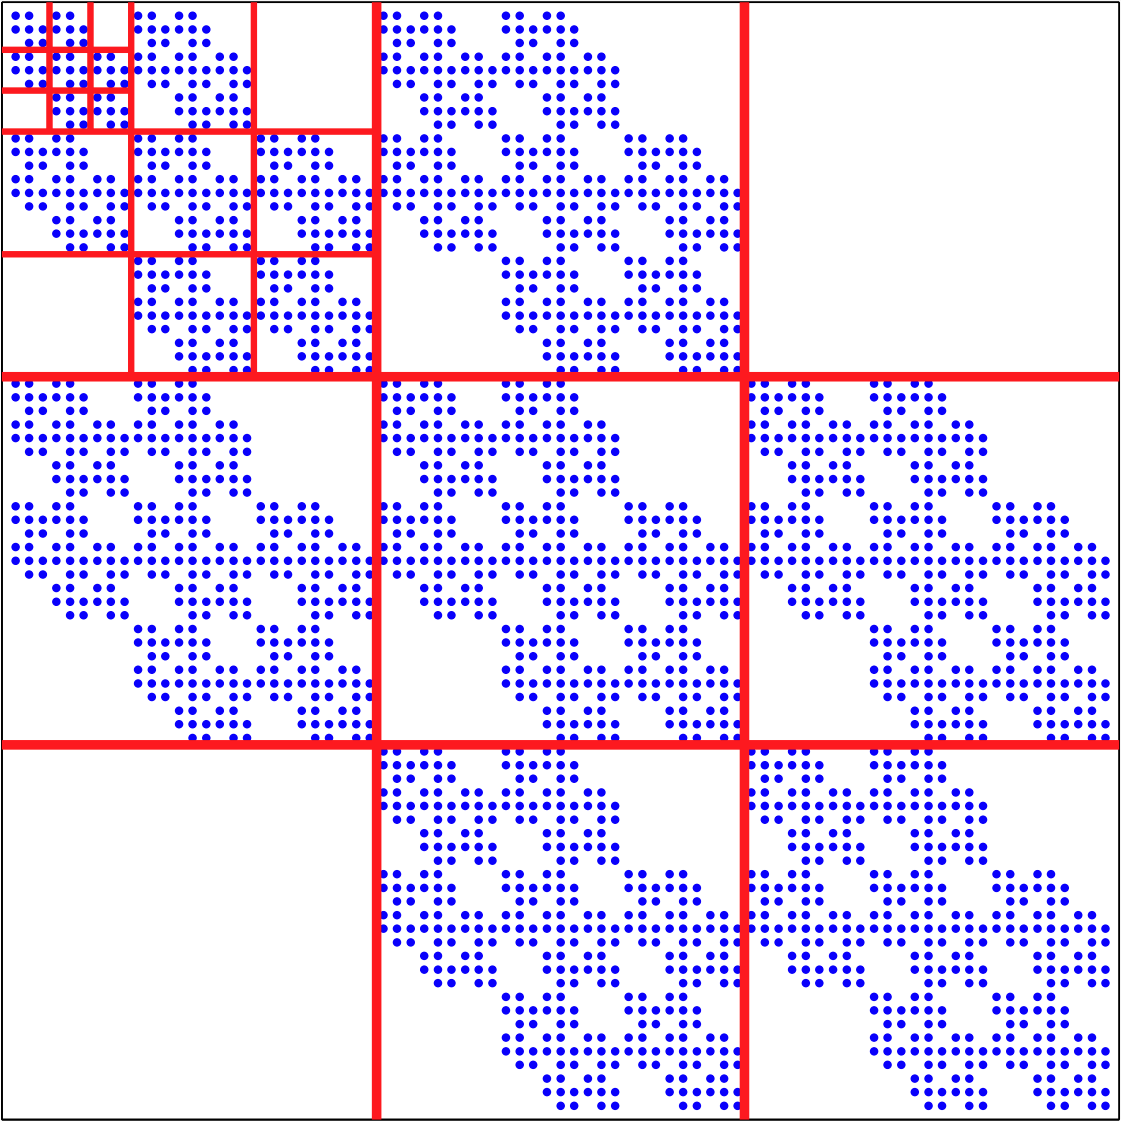
\includegraphics[width=0.5\textwidth]{figures/kronecker_adj_matrix.png}
    \caption{The adjacency matrix of the $4^{th}$ Kronecker power of a matrix. Dots are non-zero matrix entries, white space represents zeroes. \cite{Edu2010KroneckerLeskovec}}
    \label{fig:kronecker_matrix}
\end{figure}

By nature of their discrete creation process, Kronecker graphs exhibit a "staircase effect" in various metrics such as degree distribution and network value. The solution is to add randomness to the creation process to form stochastic Kronecker graphs. This variant works as follows. The adjacency matrix of the initiator graph now becomes a probability matrix. Each value $[0,1]$ denotes the probability that the edge is present. Apply the Kronecker graph creation process as usual. The end result then defines a probability distribution over all graphs. One can then simply sample an instance from this distribution.\cite{Edu2010KroneckerLeskovec}

As we are interested in generating synthetic graphs given a certain specification, the question now becomes how to tune the Kronecker creation process. Leskovec et al. \cite{Edu2010KroneckerLeskovec} describe an optimization process that aims to find an initiator matrix that has the highest likelihood to produce the adjacency matrix of a given real graph. The idea is that if the adjacency matrices of the synthetic graph and the real graph are similar then the global statistical properties over these graphs will also match. An implementation of this process called KronFit is available as open-source software as part of the Stanford Network Analysis Platform (SNAP). \cite{Leskovec2016SNAP:Library}

A clear advantage of Kronecker graphs is that one can generate graphs exhibiting desirable structural properties also found in real-world networks "from nothing" and that one can also generate synthetic graphs matching a given real-world graph by carefully choosing the initiator matrix. However, Kronecker graphs are not an all-in-one solution as they do not solve the problems of generating nodes of various types, generating different kinds of relationships and generating node attribute values. Assigning attribute values randomly to nodes would violate sensible correlations such as persons having friends within the same age group as themselves. Either one would need to graft labels, predicates and attribute values onto a Kronecker graph after-the-fact or the graph generation process somehow needs to account for attribute correlations and node type and predicate distributions.

\section{MAGs}
The multiplicative attribute graph (MAG) model is a stochastic network model that captures the interactions between node attributes and the network structure. \cite{Kim2012MultiplicativeNetworks} It only considers nodes with categorical attributes. In the MAG model, categorical node attributes have affinities to compute the probability of a link in the network. Affinities can be positive, such as shared interests increasing the probability of a link, or negative, such as same gender decreasing the probability of a relationship link. Formally, each categorical attribute has a square affinity matrix where the distinct categorical values form both the rows and the columns. Each cell of the matrix then stores the probability $p_{ij} \in (0,1)$ for a pair of nodes to form a link, given given attribute value $i$ of the first node and the value $j$ of the second node. The total link probability between two nodes is then the product of all the selected cells of the affinity matrices of the attributes of the nodes. The MAG model was proved \cite{Kim2012MultiplicativeNetworks} to capture patterns observed in real-world networks, such as power-law distributions, small diameters, unique giant connected component and local clustering of the edges.
Once a set of nodes with categorical attribute values is generated and a set of affinity matrices is constructed, the MAG model can be applied to generate the final graph. Affinity matrices can possible be manually constructed, but much more interesting and less tedious is to estimate the affinity matrices from a given graph. More specifically, given a network one wants to estimate the parameters of the distributions used to generate the node attribute values as well as the affinity matrices. An algorithm called MAGFit \cite{KimModelingModel} was developed with this purpose and is available as open-source software as part of the Stanford Network Analysis Platform (SNAP). \cite{Leskovec2016SNAP:Library} Unfortunately, MAGFit assumes that each node attribute takes the value $0$ or $1$ and follows a Bernoulli distribution, such that each affinity matrix is $2$ by $2$. This limits the applicability of the MAGFit algorithm in practice where synthetic graph nodes are expected to have realistic and usable values. Also, the MAG model does not tackle the problem of non-categorical node attributes.

\section{GScaler}
GScaler \cite{ZhangGSCALER:Graph} is a method for scaling an existing graph, analogous to DNA shotgun sequencing. GScaler works as follows. First, for each node in the input graph generate two pieces: a node with incoming edges and a node with outgoing edges. The result of this step is two bags (multisets) of pieces, one containing only pieces with incoming edges, and one containing only pieces with outgoing edges. Both bags are then scaled, ensuring the proportion of the pieces stays the same. After the scaling step it is possible the number of edges is incorrect, so the in- or out-degree of a few nodes can be adjusted in order to correct this. The pieces are then connected back to form nodes again, while making sure that the proportion of each node with a given combination of in- and out-degree stays the same. These nodes are then again connected together, ensuring that the proportion of the pairs of nodes $A$, $B$ where node $A$ has a certain in- and out-degree and node $B$ has a certain in- and out-degree stays the same. Once all nodes are connected back together, the result is a scaled graph. It must be noted that this whole process is never perfect; in each step a solution is chosen that is as optimal as possible, where the optimization is done using the Manhattan distance. GScaler produces graphs more similar to the original graph than a method like stochastic Kronecker graphs, but just like Kronecker graphs it only generates the graph structure and does not account for node attributes. Also, the GScaler algorithm does not account for graphs that have multiple node types and where relations may only be valid between nodes of certain types.

\section{DataSynth}
